\documentclass[12pt]{article}
\usepackage[margin=2.5cm]{geometry}
\usepackage{enumerate}
\usepackage{amsfonts}
\usepackage{amsmath}
\usepackage{fancyhdr}
\usepackage{amsmath}
\usepackage{amssymb}
\usepackage{amsthm}
\usepackage{mdframed}
\usepackage{graphicx}
\usepackage{subcaption}
\usepackage{adjustbox}
\usepackage{listings}
\usepackage{xcolor}
\usepackage{courier}
\usepackage[utf]{kotex}
\usepackage{hyperref}

\definecolor{codegreen}{rgb}{0,0.6,0}
\definecolor{codegray}{rgb}{0.5,0.5,0.5}
\definecolor{codepurple}{rgb}{0.58,0,0.82}
\definecolor{backcolour}{rgb}{0.95,0.95,0.92}

\lstdefinestyle{mystyle}{
    backgroundcolor=\color{backcolour},
    commentstyle=\color{codegreen},
    keywordstyle=\color{magenta},
    numberstyle=\tiny\color{codegray},
    stringstyle=\color{codepurple},
    basicstyle=\ttfamily\footnotesize,
    breakatwhitespace=false,
    breaklines=true,
    captionpos=b,
    keepspaces=true,
    numbers=left,
    numbersep=5pt,
    showspaces=false,
    showstringspaces=false,
    showtabs=false,
    tabsize=1
}

\lstset{style=mystyle}

\pagestyle{fancy}
\renewcommand{\headrulewidth}{0.4pt}
\lhead{CSC 369}
\rhead{Worksheet 2 Solution}

\begin{document}
\title{CSC 369 Worksheet 2 Solution}

\maketitle

\bigskip

\section{Homework (Simulation)}

\begin{enumerate}[1.]
    \item

    \bigskip

    I need to create process trees at each step when the command
    \texttt{./fork.py -s 10} is run.

    \bigskip

    \begin{center}
    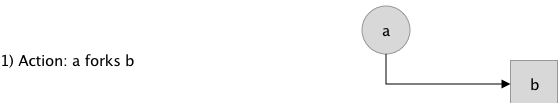
\includegraphics[width=\linewidth]{images/worksheet_2_solution_1.png}
    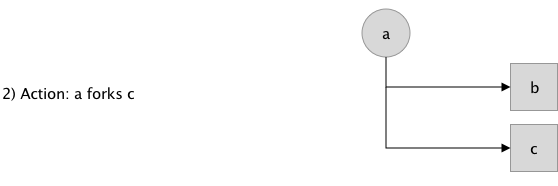
\includegraphics[width=\linewidth]{images/worksheet_2_solution_2.png}
    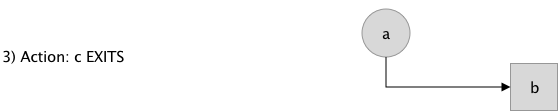
\includegraphics[width=\linewidth]{images/worksheet_2_solution_3.png}
    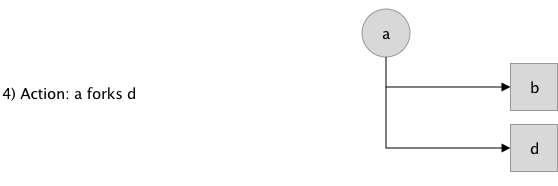
\includegraphics[width=\linewidth]{images/worksheet_2_solution_4.png}
    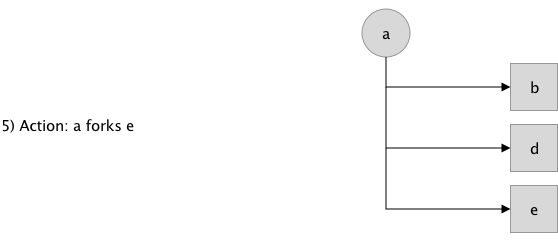
\includegraphics[width=\linewidth]{images/worksheet_2_solution_5.png}
    \end{center}

    \underline{\textbf{Notes}}

    \begin{itemize}
        \item \textbf{fork()}
        \begin{itemize}
            \item Is used to create a new process
            \item \textbf{Creator} $\to$ parent process
            \item \textbf{Newly Created} $\to$ child process
            \item Child process is nearly identical to parent process
        \end{itemize}

        \item \textbf{exec()}

        \begin{itemize}
            \item Allows a child to break free from its similarity to its parent and execute an entirely new program.
        \end{itemize}


        \item \textbf{wait()}
        \begin{itemize}
            \item Is used to let parent code delay its execution until the child finishes
            executing.
            \item Makes the output deterministic
        \end{itemize}
    \end{itemize}

    \item

    \bigskip

    I need to write what the resulting final process trees will look like as the
    fork-percentage changes. Here I ran command (\texttt{./fork.py -s 10 -a 10 -f 0.1} and \texttt{./fork.py -s 10 -a 10 -f 0.9})

    \underline{\textbf{Notes}}

    \begin{itemize}
        \item \texttt{./fork.py -s 10 -a 10 -f 0.1}

        \begin{center}
        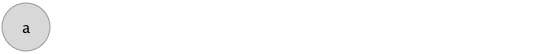
\includegraphics[width=\linewidth]{images/worksheet_2_solution_6.png}
        \end{center}

        \item \texttt{./fork.py -s 10 -a 10 -f 0.9}

        \begin{center}
        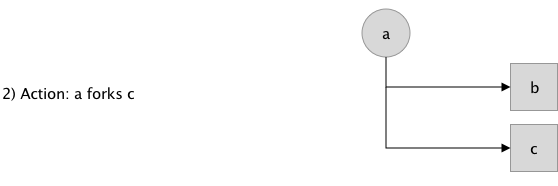
\includegraphics[width=\linewidth]{images/worksheet_2_solution_7.png}
        \end{center}

        \begin{center}
        \end{center}
    \end{itemize}

    Based on the diagram above, I can deduce that the lower the fork percentage,
    the more likely that \texttt{exit()} is executed by the childmost process, and the
    final tree will either have a single node or none.

    \bigskip

    On the other hand, the higher the fork-percentage is, the more likely that \texttt{fork()}
    is executed by the childmost process, and the final tree will have nodes that are deeply nested.

    \item

    I need to fill out blank entries created by the command (\texttt{./fork.py -t})

    \begin{center}
    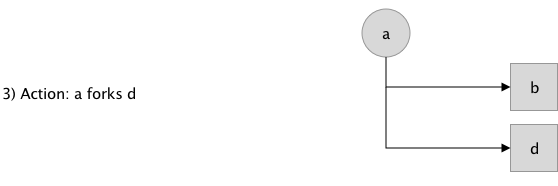
\includegraphics[width=0.7\linewidth]{images/worksheet_2_solution_8.png}
    \end{center}

    \item

    I need to write what happens when a child exits; what happens to its
    children in the process tree.

    \bigskip

    When a child exists, all of its children will also exit.

    \bigskip

    I am not sure what happens when \texttt{-R} flag is used.

    \begin{mdframed}
    \underline{\textbf{Correct Solution}}

    \bigskip

    I need to write what happens when a child exits; what happens to its
    children in the process tree.

    \bigskip

    \color{red}When a child exists, its parentmost child, along with its children,
    will be attached to the parentmost node\color{black}

    \bigskip

    \begin{center}
    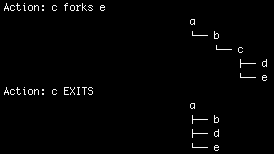
\includegraphics[width=0.7\linewidth]{images/worksheet_2_solution_9.png}
    \end{center}

    \bigskip

    \color{red}When \texttt{-R} flag is used (i.e \texttt{./fork.py -A a+b,b+c,c+d,c+e,c- -R}) and
    a child exists, its parentmost child, along with its children will be attached to
    the parent node of the child that exits\color{black}

    \bigskip

    \begin{center}
    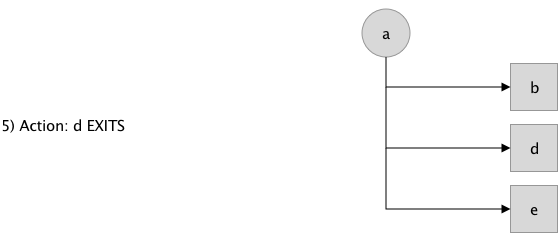
\includegraphics[width=0.7\linewidth]{images/worksheet_2_solution_10.png}
    \end{center}


    \end{mdframed}

    \item

    I need to write down the final tree by looking at the series of actions generated
    (here, the command \texttt{./fork.py -F} is used).

    \bigskip

    \begin{center}
    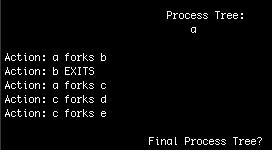
\includegraphics[width=0.7\linewidth]{images/worksheet_2_solution_11.png}
    \end{center}

    \bigskip

    \underline{\textbf{Answer:}}

    \bigskip

    \begin{center}
    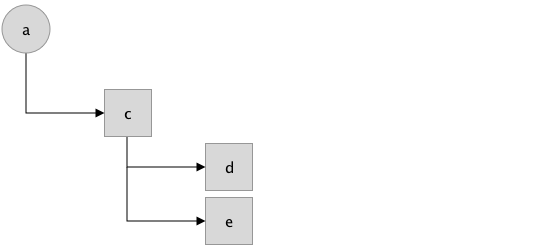
\includegraphics[width=0.7\linewidth]{images/worksheet_2_solution_12.png}
    \end{center}

    \item

    First, I need to fill the actions that took place given the final process tree.

    \bigskip

    \begin{center}
    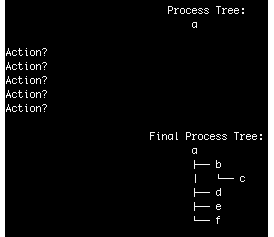
\includegraphics[width=0.7\linewidth]{images/worksheet_2_solution_13.png}
    \end{center}

    Given the final diagram, the missing actions are:

    \begin{enumerate}[1.]
        \item Action: a forks b
        \item Action: b forks c
        \item Action: a forks d
        \item Action: a forks e
        \item Action: a forks f
    \end{enumerate}

    Second, I need to write whether I can determine the exact actions that took place,
    and write where can I tell and cannot tell.

    \bigskip

    No. I cannot tell exact actions that took place. I can tell what happened upto
    the latest visible node in the diagram (e.g a, b, c, d, e, f in above diagram), but I cannot tell
    actions that took place afterwards (e.g. Action: f forks g, Action: a forks h, Action: h EXITS, and Action: g EXITS).

\end{enumerate}

\newpage

\section{Homework (Code)}

\begin{enumerate}[1.]
    \item

    Let $x = 1000$.

    \bigskip

    First, I need to write the value of the variable $x$ in the child process.

    \bigskip

    The value of $x$ in child process is the same as the parent (source code is provided in \texttt{question\_7\_part\_1.c}).

    \bigskip

    \begin{center}
    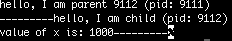
\includegraphics[width=0.5\linewidth]{images/worksheet_2_solution_14.png}
    \end{center}

    \bigskip

    Second, I need to write what happens to variable $x$ when both child and the
    parent change the value of $x$ (source code is provided in \texttt{question\_7\_part\_2.c}).

    \bigskip

    When the value of $x$ is changed in both child and parent, each possess their own values
    as if it's their own.

    \bigskip

    \begin{center}
    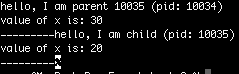
\includegraphics[width=0.5\linewidth]{images/worksheet_2_solution_15.png}
    \end{center}


    \bigskip

    \underline{\textbf{Notes}}

    \begin{itemize}
        \item C file can be compiled via command \texttt{gcc -o OUTPUT\_FILE\_NAME SOURCE\_FILE\_NAME.c}
    \end{itemize}
\end{enumerate}

\end{document}